% !TeX root = main.tex
\chapter{Introduction}\label{chap:Intro}
Physical motions exhibit a profound connection with Lie groups, appearing in diverse realms such as classical mechanics, quantum mechanics, and special relativity. This connection is not merely a matter of nomenclature but reflects an underlying and fundamental structure. While group operations are inherently interesting, the existence of a manifold equipped with a group structure -- a Lie group -- elevates this interest to a new level. Although abstract, the study of systems through the lens of Lie theory offers deeper insights into their intrinsic structure, enabling the development of more efficient and elegant control strategies.

The application of Lie groups to control theory aligns closely with geometric control theory \citep{Bullo2004}, which seeks to unify the tools of differential geometry with control problems. Instead of relying on local Euclidean charts, geometric control operates directly within the inherent manifold's structure. Similarly, our objective in this work is to design a control strategy that leverages the Lie group structure of the system, embracing its geometric and algebraic properties.

At the core of this work lies the development of a vector field guidance strategy tailored to systems with an intrinsic matrix Lie group structure. Vector field-based approaches have proven versatile in controlling various robotic systems, providing a unified framework that integrates path planning, trajectory generation, and control \citep{goncalves2010vectorfield,yao2021singularity,Rezende2022,Gao2022,nunes2023quadcopter,yao2022topological,Chen2025}. This unified framework allows for constructing a path between an initial and final configuration, generating a guidance signal for the system, and ensuring that the system follows the desired trajectory.

Our work builds upon the results of \citet{Rezende2022}, which introduced a vector field guidance strategy in Euclidean space based on the parametric representation of curves. Using this as a foundation, we extend the strategy to systems represented as matrix Lie groups. To establish this connection, we summarize the key properties and results of \citet{Rezende2022}, which serve as the groundwork for our generalization. Throughout the text, we use examples to illustrate and clarify the parallels and distinctions between the two approaches, ensuring the continuity and coherence of our contributions.

One particularly compelling application of extending vector fields to matrix Lie groups is the control of systems capable of simultaneous motion in both position and orientation, which can be addressed by considering the group $\text{SE}(3)$ within our framework. Omnidirectional unmanned aerial vehicles (UAVs), such as those illustrated in \cref{fig:omnidirectionaldrone}, exemplify such capabilities, and research in this domain is rapidly advancing \citep{kamel2018voliro,Aboudorra2023,HamandiOmni}. For instance, in \citet{hamandi2021design} a comprehensive review of multirotor designs is provided, identifying critical factors that enable omnidirectional motion. These capabilities are particularly relevant for tasks requiring complex maneuvers, such as tracking paths that involve intricate trajectories. This is especially important when UAVs are equipped with tools like drills, where precise positioning is needed to achieve target poses while avoiding environmental collisions. Our approach facilitates such tasks by controlling the linear and angular velocities of the UAV. Additionally, another notable application of $\text{SE}(3)$ is in robotic manipulators, where our method can control the end effector's linear and angular velocities.
\begin{figure}[ht]
    \centering
    % \def\svgwidth{\columnwidth}
    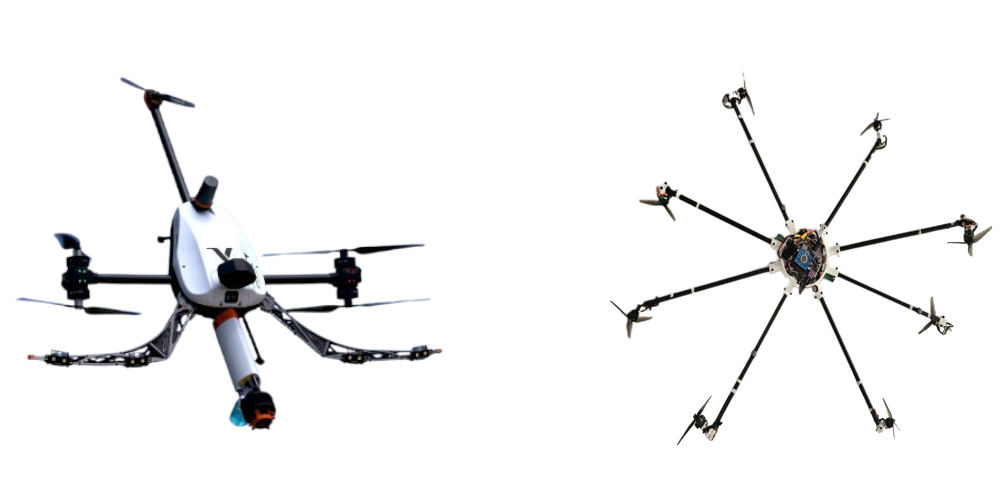
\includegraphics[width=.8\columnwidth]{figures/example_omnidirecitonal_wobg.png}
    \caption{One application of our strategy is the control of omnidirectional drones, like (left) a Voliro drone (image taken from \url{https://voliro.com}) and (right) the design from \citet{HamandiOmni}. Since they accept arbitrary $6$ DoF twists, our methodology can be used to control them to track arbitrary differentiable paths in $\text{SE}(3)$.}
    \label{fig:omnidirectionaldrone}
\end{figure}

Although these applications demonstrate the versatility of our approach, it is important to emphasize that our primary focus is not on specific use cases but on the theoretical foundation itself. As will become evident, our generalization not only enables the use of vector fields on Lie groups but also reveals that the vector field strategy in Euclidean space offers more flexibility than previously recognized. To encapsulate our intent, we draw on the perspective of Francesco Bullo, who states that ``the areas of overlap between mechanics and control possess the sort of mathematical elegance that makes them appealing to study, independently of applications.'' \citep{Bullo2004}.

To illustrate the potential of our generalization, we provide two application scenarios. The first is a kinematic control simulation of a system in $\text{SE}(3)$, where the goal is to converge to and circulate along a predefined curve within the group. This simulation offers a concrete example of how our theoretical results can be practically applied and visualized. Within the kinematic scenario, we also simulate a system in $\text{SO}^+(3,1)$. While this does not provide a visual representation of the strategy, it demonstrates its generality. The second scenario involves a collaborative simulation in which six agents manipulate a cylindrical object with unknown properties to track a target curve. In this case, we work within the group $\mathbb{R}^3\times\text{SO}(3)$, where translation and rotation are treated as independent motions. Due to the object's unknown parameters, we employ an adaptive control strategy to estimate these properties and achieve control. Here, our vector field strategy serves as a higher-level controller, providing desired velocity inputs to a lower-level dynamic controller responsible for tracking these velocities. This simulation highlights the adaptability of our approach to dynamic scenarios, particularly those requiring parameter estimation and adaptation.

Although not essential to understanding this work, we provide a brief background on its development. Motivated by an interest in nonlinear dynamic control techniques from graduate coursework, we sought to extend previous assignments and explore their broader applications. During this process, we encountered \citet{Culbertson2021}, which addressed adaptation in robotic manipulation. This led us to investigate whether their approach could be adapted to a vector field framework based on \citet{Rezende2022}. Building on this, we explored the inclusion of orientation, culminating in a formulation in $\mathbb{R}^3\times\text{SO}(3)$, later published in \citet{Pessoa2024}. Observing its properties, we identified a broader generalization for systems in matrix Lie groups, leading to the more general vector field guidance strategy presented here, currently under review at \textit{Automatica}.

The previous disclaimer not only provides insight into how this work evolved but also explains certain modifications made to this text. Here, we focus on the generalized vector field approach for systems represented as matrix Lie groups, treating \citet{Pessoa2024} as an application of this broader framework. Consequently, our presentation adopts a non-chronological order. We begin with the more general case, as it offers a clearer conceptual foundation, and then demonstrate its application to specific scenarios. Some portions of the text from \citet{Pessoa2024} have been rewritten to better fit the context of this work and may differ from the original. Furthermore, we expand on certain derivations and proofs from both works to provide deeper insights.
\section{Summary of contributions}
The main contributions of this work can be summarized as follows:
\begin{itemize}
    \item Development of a novel vector field guidance strategy applicable to systems with an inherent matrix Lie group structure;
    \item Implementation framework for $\text{SE}(3)$ systems, providing all necessary tools for practical application of the proposed strategy;
    \item Validation through kinematic simulations in $\text{SE}(3)$ and $\text{SO}^+(3,1)$, demonstrating the theoretical results and their practical implications;
    \item Design of an adaptive control strategy for collaborative simulations in $\mathbb{R}^3 \times \text{SO}(3)$, where the vector field guidance strategy generates reference velocities for dynamic control.
\end{itemize}

\section{Publications}
In this section we highlight the publications that culminated into the present work
\begin{itemize}
    \item \textbf{Pessoa, F. B. A.}; Pimenta, L. C. A. . Vector Field Based Adaptive Control for Collaborative Manipulation. In: \textbf{XXV Congresso Brasileiro de Automática}, 2024, Rio de Janeiro. Anais do XXV Congresso Brasileiro de Automática, 2024
    \item \textbf{Bartelt, F.}; Gonçalves, V. M.; Pimenta, L. C. A. . Constructive Vector Fields for Path Following in Matrix Lie Groups. \textbf{Submitted to Automatica}, 2025.
\end{itemize}
\section{Structure of the text}
This work is organized as follows:
\begin{itemize}
    \item \chapref{chap:literature-review}\\
    We review the formulation of vector fields and the application of Lie theory across various domains.
    \item \chapref{ch:background}\\
    This chapter revisits the vector field guidance strategy in Euclidean space, provides the necessary background on Lie groups and Lie algebras, and introduces the foundational concepts of adaptive control.
    \item \chapref{ch:vector_field}\\
    We present the generalization of the vector field guidance strategy to matrix Lie groups, detailing its application to kinematic control in exponential Lie groups and providing the necessary tools for implementation in $\text{SE}(3)$.
    \item \chapref{ch:collaborative}\\
    This chapter introduces the system model, the lower-level controller, and the adaptive control strategy for a collaborative manipulation scenario.
    \item \chapref{ch:results}\\
    We present the details and results of simulations for both explored scenarios.
    \item \chapref{ch:conclusion}\\
    The text concludes with a summary of the findings and a discussion of potential directions for future research.
\end{itemize}

